\documentclass[a4paper, 11pt]{space}
\usepackage{siunitx}
\usepackage{tikz}
\usetikzlibrary{calc}
\usepackage{framed}

\newenvironment{example}[0]{\begin{framed}{\bf Example:}}{\end{framed}}
\author{Marijn van Vliet}
\title{Orbital maneuvering}

\begin{document}
\maketitle

\section{Orbital speed}\label{orbital_speed}

The following formula describes the speed of a spacecraft orbiting a planet or moon:
\begin{center}
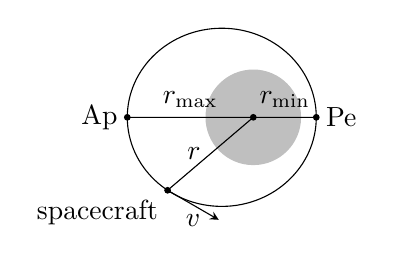
\begin{tikzpicture}[>=stealth]{width=8}
    % Define parameters of orbit
    \def\Pe{0.8};
    \def\Ap{1.6};

    % Draw planet
    \draw[fill, gray!50] (0,0) circle (0.6);

    % Draw center of planet
    \draw[fill] (0,0) circle (1pt);

    % Draw orbit of craft
    \draw ({-(\Ap-\Pe)/2},0) ellipse ({(\Ap+\Pe)/2} and {sqrt(\Ap*\Pe)});

    % Draw Pe and Ap
    \draw[fill] (\Pe,0) circle (1pt) node[right]{Pe} -- node[above]{$r_{\mathrm{min}}$}(0,0);
    \draw[fill] (-\Ap,0) circle (1pt) node[left]{Ap} -- node[above]{$r_{\mathrm{max}}$}(0,0);

    % Draw spacecraft
    \draw[fill] (0,0) -- node[left]{$r$} 
                ($({-(\Ap-\Pe)/2},0) + (-125:{(\Ap+\Pe)/2} and {sqrt(\Ap*\Pe)})$) 
                circle (1pt)
                node[below left]{spacecraft};

    % Draw velocity vector
    \draw[->] ($({-(\Ap-\Pe)/2},0) + (-125:{(\Ap+\Pe)/2} and {sqrt(\Ap*\Pe)})$) 
              -- node[below]{$v$} ++(-30:0.75);

\end{tikzpicture}
\end{center}
\begin{align}
    v^2 &= MG \left( \frac{2}{r} - \frac{2}{r_\mathrm{min} + r_\mathrm{max}} \right),
\end{align}

where $M$ is the mass of the planet in kilograms, $G$ is the gravitational constant (\num{6.67384E-11}), $r_\mathrm{min}$ is the distance from the periapsis to the center of the planet in meters, $r_\mathrm{max}$ is the distance from the apoapsis to the center of the planet in meters, $r$ is the distance from the current position of the craft to to the center of the planet in meters and $v$ is the velocity of the craft in meters per second. 

Because $MG$ is generally known at a better precision than $M$ and $G$ separately, the so called gravitational parameter $\mu=MG$ is usually listed directly in planetary almanacs, such as the KSP wiki. Also, because the average of the periapsis and apoapsis, called the semi-major-axis, is used in a lot of formulae, we denote $a = \frac{r_\mathrm{min} + r_\mathrm{max}}{2}$. Substituting $\mu$ and $a$ in the formula above gives:

\begin{align}
	v^2 &= \mu \left(\frac{2}{r} - \frac{1}{a} \right).
\end{align}

Finally, as we're usually interested in the velocity $v$ and not $v^2$, we take the root:

\begin{align}
	v &= \sqrt{\mu \left(\frac{2}{r} - \frac{1}{a} \right)}.
\end{align}

\begin{example}
    Bob is in orbit around Kerbin. His instruments show that his periapsis is at \unit[80]{km}, his apoapsis is at \unit[160]{km} and his current altitude is \unit[119.253]{km}. Note that these instruments tell us the altitudes relative to the surface of Kerbin and the formula wants them as distances to the center of Kerbin. We can read on the KSP wiki that the radius of Kerbin is \unit[600]{km}. To calculate the semi-major-axis of Bob's orbit, we add the radius of Kerbin to Bob's periapsis and apoapsis:
\[ a = \frac{r_\mathrm{min} + r_\mathrm{max}}{2} = \frac{(80000 + 600000) + (160000 + 600000)}{2} = \unit[720000]{m} = \unit[720]{km}.
\]
We also read in the wiki that the gravitational parameter $\mu$ of Kerbin is \num{3.5316E12}. The current velocity of Bob's craft should be:
\[ v = \sqrt{\mu \left(\frac{2}{r} - \frac{1}{a} \right)} = \sqrt{\num{3.5316E12} \left(\frac{2}{119253+600000} - \frac{1}{720000}\right)} \approx \unit[2217]{m/s}.
\]
You can check in KSP to verify.
\end{example}

\section{Speed in circular orbits}\label{circular_orbit}

When a craft is in a circular orbit, the periapsis and apoapsis of the orbit, as well as the current altitude of the craft, are all the same. This simplifies the formula for calculating the speed of the craft:

\begin{center}
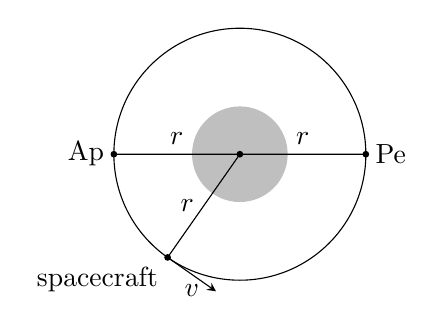
\begin{tikzpicture}[>=stealth]{width=8}
    % Define parameters of orbit
    \def\r{1.6};

    % Draw planet
    \draw[fill, gray!50] (0,0) circle (0.6);

    % Draw center of planet
    \draw[fill] (0,0) circle (1pt);

    % Draw orbit of craft
    %\draw ({-(\Ap-\Pe)/2},0) ellipse ({(\Ap+\Pe)/2} and {sqrt(\Ap*\Pe)});
    \draw (0,0) circle (\r);

    % Draw Pe and Ap
    \draw[fill] (\r,0) circle (1pt) node[right]{Pe} -- node[above]{$r$}(0,0);
    \draw[fill] (-\r,0) circle (1pt) node[left]{Ap} -- node[above]{$r$}(0,0);

    % Draw spacecraft
    \draw[fill] (0,0) -- node[left]{$r$} (-125:\r)
                circle (1pt) node[below left]{spacecraft};

    % Draw velocity vector
    \draw[->] (-125:\r) -- node[below]{$v$} ++(-35:0.75);

\end{tikzpicture}
\end{center}
\begin{align}
    v^2 &= MG \left( \frac{2}{r} - \frac{2}{r_\mathrm{min} + r_\mathrm{max}} \right), \\
    v^2 &= MG \left( \frac{2}{r} - \frac{2}{r + r} \right), \\
    v^2 &= MG \left( \frac{1}{r} \right), \\
    v &= \sqrt{\frac{\mu}{r}}.
\end{align}

\begin{example}
    Bob decides to circularize his orbit around Kerbin. Currently his periapsis is \unit[80]{km} and his apoapsis is \unit[160]{km}. He decides to burn at apoapsis to raise his periapsis.

\begin{center}
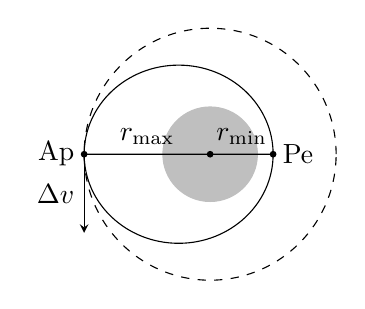
\begin{tikzpicture}[>=stealth]{width=8}
    % Define parameters of orbit
    \def\Pe{0.8};
    \def\Ap{1.6};
    \def\DesiredR{1.6};

    % Draw planet
    \draw[fill, gray!50] (0,0) circle (0.6);

    % Draw center of planet
    \draw[fill] (0,0) circle (1pt);

    % Draw orbit of craft
    \draw ({-(\Ap-\Pe)/2},0) ellipse ({(\Ap+\Pe)/2} and {sqrt(\Ap*\Pe)});

    % Draw Pe and Ap
    \draw[fill] (\Pe,0) circle (1pt) node[right]{Pe} -- node[above]{$r_\mathrm{min}$}(0,0);
    \draw[fill] (-\Ap,0) circle (1pt) node[left]{Ap} -- node[above]{$r_\mathrm{max}$}(0,0);

    % Draw desired orbit
    \draw[dashed] (0,0) circle(\DesiredR);

    % Draw velocity vector
    \draw[->] (-\Ap, 0) -- node[left]{$\Delta v$} ++(0, -1);
\end{tikzpicture}
\end{center}
    
How much $\Delta v$ should he burn for? To answer this, we need to know how fast he's going when he reaches apoapsis and how fast he \emph{should} be going in order to obtain a circular orbit. His speed at apoapsis will be:
\[ v_\mathrm{Ap} = \sqrt{\mu \left(\frac{2}{r} - \frac{1}{a} \right)} = \sqrt{\num{3.5316E12} \left(\frac{2}{160000+600000} - \frac{1}{720000}\right)} \approx \unit[2095]{m/s},
\]
and to obtain a circular orbit, he \emph{should} be going:
\[ v_\mathrm{circ} = \sqrt{\frac{\mu}{r}} = \sqrt{\frac{\mu}{160000+600000}} \approx \unit[2156]{m/s}.
\]
So his burn must increase his speed with $v_\mathrm{circ} - v_\mathrm{Ap} = 2156 - 2095 = \unit[61]{m/s}$.
\end{example}

\section{Orbital period}\label{orbital_period}

The formula for the orbital period of a spacecraft orbiting a planet is:
\[ T = 2 \pi \sqrt{\frac{a^3}{\mu}}, \]

where $a$ is the semi-major-axis (see \autoref{orbital_speed}), $\mu$ is the gravitational parameter of the planet (see also \autoref{orbital_speed}), and $T$ is the time it takes to complete one orbit in seconds.

\begin{example}
    Mission control wants to put a satellite into orbit around Kerbin, so that it always floats exactly above the KSP; a so called synchronous orbit. In this special circular orbit, the satellite takes exactly as long to complete an orbit as Kerbin does to rotate around her axis, or in other words, the orbital period of the satellite is exactly one Kerbin day. How fast should the satellite be going and at which altitude should it be flying? The KSP wiki tells us one Kerbin day is \unit[21600]{s}. If the orbital period of the satellite should be equal to that, the semi-major-axis of its orbit should be:
\begin{align*}
    T &= 2 \pi \sqrt{\frac{a^3}{\mu}}, \\
    \sqrt{\frac{a^3}{\mu}} &= \frac{T}{2\pi}, \\
    \frac{a^3}{\mu} &= \frac{T^2}{4\pi^2}, \\
    a^3 &= \frac{\mu T^2}{4\pi^2}, \\
    a &= \sqrt[3]{\frac{\mu T^2}{4\pi^2}} = \sqrt[3]{\frac{\num{3.5316E12} \cdot 21600^2}{4\pi^2}} \approx \unit[3468751]{m}.
\end{align*}

Since in a circular orbit, the periapsis and apoapsis are equal, the semi-major-axis is also equal to the altitude at which the satellite will be flying. However, this is measured as the distance to the center of the planet, while generally in KSP, the altitude is measured relative to the surface of the planet. The KSP wiki tells us the radius of Kerbin is \unit[600]{km}, so the altitude of a satellite in Kerbin-synchronous orbit is $3468751 - 600000 = \unit[2868751]{m} = \unit[2868.751]{km}$. The speed at which it will be flying (see \autoref{circular_orbit}) is:
\begin{align*}
    v = \sqrt{\frac{\mu}{r}} = \sqrt{\frac{\num{3.5316E12}}{3468751}} \approx \unit[1009]{m/s}.
\end{align*}

\end{example}

\end{document}
